% This is LLNCS.DEM the demonstration file of
% the LaTeX macro package from Springer-Verlag
% for Lecture Notes in Computer Science,
% version 2.4 for LaTeX2e as of 16. April 2010
%
\documentclass{llncs}
%
\usepackage{makeidx}  % allows for indexgeneration
\usepackage{listings}
\usepackage{graphicx}

%
\begin{document}
%
\frontmatter          % for the preliminaries
%
\pagestyle{headings}  % switches on printing of running heads
% \addtocmark{Hamiltonian Mechanics} % additional mark in the TOC
%
%
\mainmatter              % start of the contributions
%
\title{Context-Oriented J Programming}
%
\titlerunning{Context-Oriented J Programming}  % abbreviated title (for running head)
%                                     also used for the TOC unless
%                                     \toctitle is used
%
\author{Bastian Kruck}
%
\authorrunning{Bastian Kruck} % abbreviated author list (for running head)
%
%%%% list of authors for the TOC (use if author list has to be modified)
\tocauthor{Bastian Kruck}
%
\institute{Hasso-Plattner-Institut Potsdam\\
\email{bastian.kruck@student.hpi.uni-potsdam.de}}

\maketitle              % typeset the title of the contribution

\begin{abstract}
In diesem Seminar werde ich ein context-oriented programming framework in der Array-Programmiersprache J implementieren. Mit dessen Hilfe werde ich das Datenbanksystem jdb refaktorieren um Funktionalit\"aten ein und auszuschalten zu k\"onnen. So k\"onnen andere Pakete das Verhalten der Datenbank auf die jeweilige Situation optimieren. Zum Beispiel ist das importieren einer validen, sortierten Datenbank schneller, wenn die Validierung und Sortierung daf\"ur tempor\"ar ausgeschaltet wird.

\keywords{context-oriented programming, software, j programming language, array programming}
\end{abstract}
%
\section{Background}
%

Array Programming erm\"oglicht das pr\"azise Manipulieren multidimensionaler Daten. Ingenieure schreiben darin Skripte, um wegleitende Erkenntnisse aus z.B. sensorischen oder statistischen Daten zu gewinnen.

In der Array-Programming-Sprache J gibt es Namensr\"aume (�locales�) \footnote{Quelle: \url{http://www.jsoftware.com/help/dictionary/dx018.htm} und \url{http://www.jsoftware.com/help/learning/24.htm}, aufgerufen am 24.10.2014}. Diese (a) helfen Namenskollisionen zu vermeiden, (b) bieten einen G\"ultigkeitsbereich f\"ur lokale Variablen und (c) haben einen lookup-Mechanismus, der das Nachschlagen von globalen Variablen erm\"oglicht. Das Verhalten des lookup-Mechanismus wird durch eine Liste von Namensr\"aumen bestimmt (�lookup-Pfad�). Bei Benutzung einer nicht definierten Variablen wird transparent der Reihe nach versucht, diesen Namen in einem der Namensr\"aume im lookup-Pfad aufzul\"osen und bei Erfolg der gefundene Wert zur\"uckgegeben. Das funktioniert f\"ur Operanden (�Nomen�), benannte Operatoren (�Verben�) und benannte Funktionen h\"oherer Ordnung (�Adverbien� und �Konjunktionen�).
Der lookup-Mechanismus wird in J benutzt um prototypbasierte Objekt-Orientierung zu implementieren. Die Standardbibliothek (�stdlib.ijs�) implementiert daf\"ur u.a. die Hilfsmethoden \texttt{coclass}, \texttt{coinsert}, \texttt{conew} \footnote{Quelle: \url{http://www.jsoftware.com/help/learning/25.htm}, aufgerufen am 24.10.2014}.\\

\begin{description}
\item[\texttt{coclass 'Collection'}] erzeugt einen neuen Namensraum namens 'Collection' und w\"ahlt ihn als aktuell aus.
\item[\texttt{coinsert 'AbstractClass'}] h\"angt den Namensraum �AbstractClass� vorne an den lookup-Pfad vom aktuellen Namensraum. �Collection� ist nun eine Unterklasse von �AbstractClass�.
\item[\texttt{conew �Collection�}] erzeugt einen neuen (namenlosen) Namensraum und nimmt �Collection� in den lookup-Pfad auf.
\end{description}

Um in J zwischen Kontexten zu differenzieren werden bisher Verzweigungen benutzt. Zum Beispiel wird in trace.ijs abh\"angig vom Modus-Parameter (\texttt{t\_mode}) entweder die \texttt{execute}-Funktion f\"ur das Nachverfolgen (�Trace�) oder Klammern (�Parenthesis�) benutzt (siehe Listing \ref{lst-traceIjsMode}).

\begin{lstlisting}[label=lst-traceIjsMode, caption=Verzweigungen tauschen alternative Implementierungen abh\"angig vom Modus aus\, trace.ijs\, Zeile 185]
 if. 'trace' -: t_mode do.
  execute=. executet
  move   =. movet
 else.
  execute=. executep
  move   =. movep
 end.
\end{lstlisting}

J hat ein ausgereiftes Paketsystem. Es gibt Mechanismen zum Beschreiben von Abh\"angigkeiten von anderen Paketen und zum Definieren von Demos und Tests.

\texttt{jdb} ist das Standarddatenbanksystem von J. Im Paket \texttt{'data/jdb'} wird eine Implementierung bereitgestellt, die schnell und zuverl�ssig funktioniert. Eine Unterscheidung verschiedener Modi wird nicht vorgenommen (siehe Listing \ref{lst-jdbNoModi}). Sortierung findet nur zur Anfragezeit statt und die Validierung von Datensatzformat und Fremdschl\"usseln ist unausweichlich. K\"onnte man die automatischen Transaktionen abschalten, so w\"aren manuelle Transaktionsb\"undelung und schnelles Importieren m\"oglich.

\begin{lstlisting}[label=lst-jdbNoModi, caption=Im Paket \texttt{data/jdb} sind Transaktionen und die Validierung des inneren Zustands unumg\"anglich. jdb.ijs\, Zeile 1180.]
Delete=: 3 : 0
   delete y
   commit''
   dbwritetrans''
)
\end{lstlisting}

\section{Solution}
Fast alle Skripte in der J Standard-Umgebung sind innerhalb eines speziellen Namensraums formuliert. Wenn es nicht explizit angegeben ist, so ist der aktuelle Namensraum \texttt{base} und \texttt{z} der einzige Namensraum im lookup-Pfad.

J bietet gen\"ugend Reflektion, um COP zu implementieren. Es lassen sich Methoden aus einem speziellen Namensraum im Variablenbereich eines anderen ausf\"uhren sowie die Methoden eines Namensraums auflisten und ver\"andern.

\section{Impact}
\textbf{Layern von \texttt{jdb} macht J schneller und besser.} J ist eine Sprache zur Datenverarbeitung. Das Datenbanksystem stellt einen wichtigen Bestandteil der Sprachumgebung dar. Durch das Layern von \texttt{jdb} wird dieser Bestandteil beherrschbarer und m\"achtiger. Entwickler k\"innen von mehr Funktionalit\"at und von stellenweise besserer Geschwindigkeit profitieren.

%Durch layern der Bibliotheksfunktionen lassen sie sich auf die beschriebenen Kontext optimieren. M�gliche dynamische Anpassungen sind dabei:
%- die Ausf�hrlichkeit bei der Ausgabe von Zwischenergebnissen
%- die Genauigkeit bei der Verarbeitung gro�er Datenmengen (Algorithmus-Entwurf auf kleiner Datenmenge, Analyse auf den vollst�ndigen Daten)
%- das �Einfrieren� von Zust�nden, um Zwischenergebnisse von Operationen zu sehen, ohne den Zustand des Terminals zu ver�ndern
%- Anpassen des Rangs von bestimmten Operationen, um von der Analyse eines Datensatzes zur Analyse einer ganzen Tabelle �berzugehen

\textbf{Context-oriented J Programming macht die Arbeit mit Paketen in J konfliktfreier und bed\"urfnisgerechter.} Mit Context-based J Programming lassen sich Bibliotheksfunktionen auf die wechselnden Anforderungen an die Sprachumgebung dynamisch optimieren. Ein Paket, das Konsumenten eine Schnittstelle zum gezielten Ein- und Ausschalten von Funktionalit\"at bietet, erf\"ullt mehr Bed\"urfnisse von konsumierenden Paketen. Das dynamische Ein- und Ausschalten verhindert Konflikte bei der Benutzung mehrerer Pakete (der Importierer m\"ochte keine Validierung, das Wartungsfrontend schon).
	
\section{Appendix I: Proof of Concept}

Dies sind Screenshots von einer Proof-of-Concept-Implementierung vom �Einfrieren� einer Collection.

\textbf{Hilfe zur Unterstrich Notation}
Sei \texttt{obj} ein Objekt der Klasse \texttt{Class}.
\texttt{Method\_\_obj 0} ist equivalent zu \texttt{Method\_8\_ 0} wobei \texttt{8} die id von \texttt{obj} ist. \texttt{Method\_8\_} ist nicht definiert, aber \texttt{Method\_Class\_} kann aufgel\"ost werden und so wird die Methode \texttt{Method} aus dem Namensraum \texttt{Class} auf dem Object \texttt{obj} ausgef�hrt.
\\
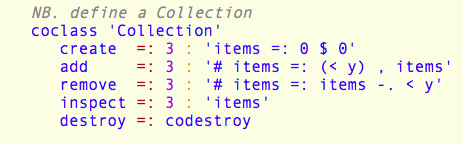
\includegraphics[width=\textwidth]{figures/1}
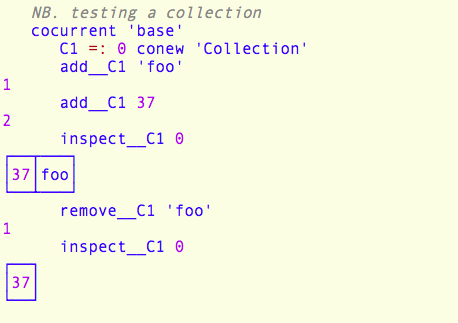
\includegraphics[width=\textwidth]{figures/2}
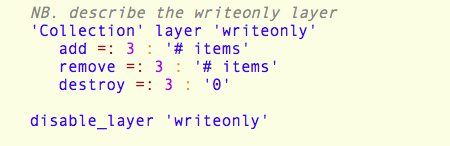
\includegraphics[width=\textwidth]{figures/3}
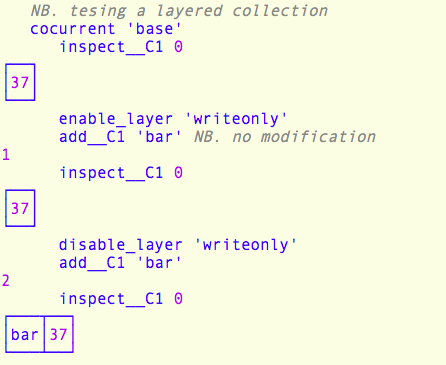
\includegraphics[width=\textwidth]{figures/4}
\clearpage
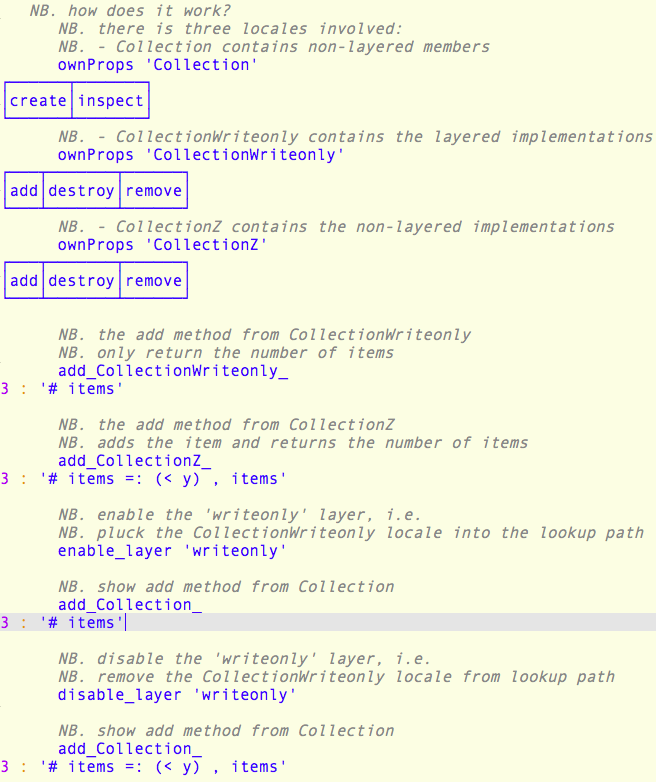
\includegraphics[width=\textwidth]{figures/5}

\end{document}
